\chapter{Einleitung}
\label{cha:einleitung}
Im Gegensatz zu den vergangenen Jahren war es die Aufgabe dieses Projektseminars Echtzeitsysteme eine Steuerung zu entwickeln, die ein Modellauto innerhalb gegebener Spuren fahren lässt. Durch eine Kamera und verschiedene Sensoren wird die Umgebung erkannt und mittels Filterungen und Regelungen in Steuerbefehle für das Fahrzeug umgewandelt.
\tod{Weiter schreiben}


\chapter{Grundlagen}
\label{cha:grundlagen}
\section{Modellauto}
\label{sec:modellauto}
evtl. Hardwaregrundlagen
\section{OpenCV}
\label{sec:openCV}
\section{ROS - Robot Operating System}
\label{sec:ros}
ROS ist ein Metabetriebssystem für Roboter, welches auf Linux basiert und in vielen Unternehmen für Steuerung von Robotern genutzt wird. Es stellt mehrere Pakete zur Verfügung, die einige nützliche Funktionen ermöglichen. Dazu gehört die Verteilung auf mehrere Systeme im Netzwerk, Paketverarbeitung und die Kommunikation zwischen den Nodes \cite{einfuehrungROS}.
Die Kommunikation findet durch ein Publish-Subscribe-System statt. Die einzelnen Nodes publishen zu  bestimmten Themen Nachrichten, deren Inhalt sich auf das Thema bezieht. So erhält man zum Thema \code{/uc\_bridge/usr} über eine Subscription Nachrichten über die Werte des rechten Abstandssensors. Auch die Steuerung des Motors und des Lenkwinkels geschieht über das puplishen von Nachrichten. 

\section{PSES Packages}
\label{sec:psespackages}

\chapter{Organisation}
\label{cha:organisation}
evtl. Schild und Licht mit rein
\section{Aufgabenverwaltung}
\label{sec:aufgabenverwaltung}
\section{Versionsverwaltung}
\label{sec:versionsverwaltung}


\chapter{Lösung}
\label{cha:loesung}
\section{Contour Detection}
\label{sec:contourDetection}
\section{\textquotedblleft Wallfollower\textquotedblright}
\label{sec:wallfollower}
\section{Hindernisvermeidung durch Spurwechsel}
\label{sec:spurwechsel}
text


\chapter{Probleme}
\label{cha:probleme}
\begin{itemize}
	\item unzuverlässiger Ultraschallsensor mit falschen Werten (in akustisch ungedämpfter Umgebung)
	\item verworfene Ansätze: Bildfilterung und Edge Detection mit Canny\\
	Contour Detection und malen des kleinsten Rechtecks
\end{itemize}
\begin{figure}[h]
	\label{fig:rechtecke}
	\centering
	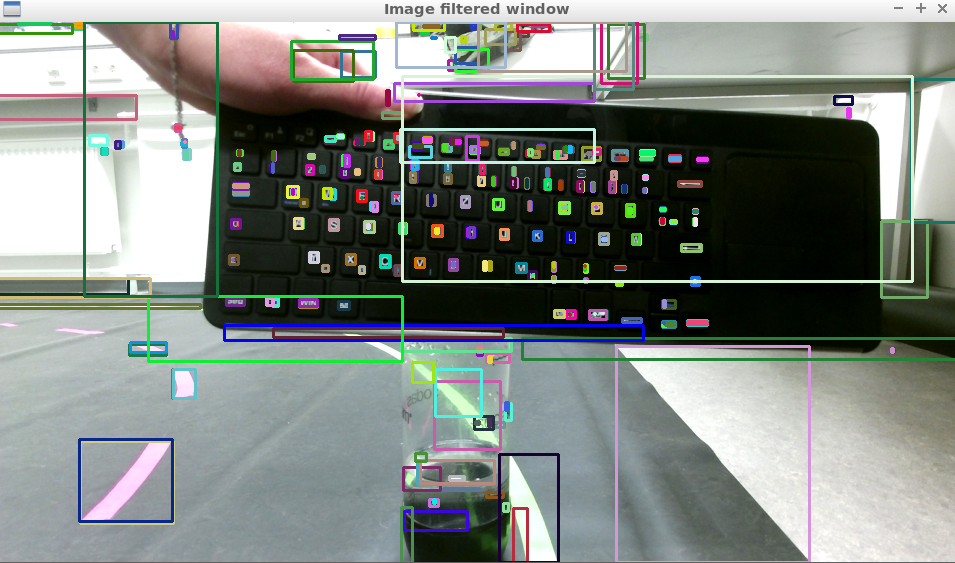
\includegraphics[width=0.7\textwidth]{images/rechtecke.png}
	\caption{Contour Detection mit kleinsten umfassenden Rechtecken}
\end{figure}
\section{Kinect und Weitwinkelkamera}
\label{sec:kinectWeitwinkel}
\begin{itemize}
	\item Farbprobleme mit Weitwinkelkamera im Vergleich zur Kinect
	\item zu wenig Bildausschnitt mit Kinect
\end{itemize}
text

